\documentclass[12pt]{article}

\title{\vspace{-3em}PHYS 161a HW 2}
\author{Michael Cardiff}
\date{\today}

%% science symbols 
\usepackage{amsmath}
\usepackage{amssymb}
\usepackage{physics}
\usepackage{slashed}

%% general pretty stuff
\usepackage{bm}
\usepackage{enumitem}
\usepackage{float}
\usepackage{graphicx}
\usepackage[margin=1in]{geometry}
\usepackage[labelfont=bf]{caption}
\usepackage{tikz}

% figures
\graphicspath{ {./figs/} }

\newcommand{\fig}[3]
{
  \begin{figure}[H]
    \centering
    \includegraphics[width=#1cm]{#2}
    \caption{#3}
  \end{figure}
}

\newcommand{\figref}[4]
{
  \begin{figure}[H]
    \centering
    \includegraphics[width=#1cm]{#2}
    \caption{#3}
    \label{#4}
  \end{figure}
}

\newcommand*\circled[1]{\tikz[baseline=(char.base)]{
            \node[shape=circle,draw,inner sep=2pt] (char) {#1};}}
\renewcommand{\L}{\mathcal{L}}
\newcommand{\D}{\partial}
\newcommand{\munu}{{\mu\nu}}
\newcommand{\sla}[1]{\slashed{#1}}

\begin{document}
\maketitle

\section*{Problem 1}
\subsection*{Part 1}

\subsection*{Part 2}

\section*{Problem 2}
\subsection*{Part 1}
The Fourier series for a function in terms of $e^{int}$ is given by:
\begin{align*}
  g(t)=\sum_{n=-\infty}^{\infty}A_n\exp(int)
\end{align*}
With the coefficient being:
\begin{align*}
  A_n=\frac{1}{2\pi}\int_0^{2\pi}g(t)e^{-int}\dd{t}
\end{align*}
Plug in $g(t)$:
\begin{align*}
  A_n&=\frac{1}{2\pi}\int_0^{2\pi}
  \qty(\frac{\pi^2}{6}-\frac12(t-\pi)^2)e^{-int}\dd{t}\\
  &=\frac\pi{12}\int_0^{2\pi}e^{-int}\dd{t}
  -\frac{1}{4\pi}\int_0^{2\pi}(t-\pi)^2e^{-int}\dd{t}\\
  &=\frac{\pi}{12}\circled{1}-\frac{1}{4\pi}\circled{2}
\end{align*}
Evaluate each integral:
\begin{align*}
  \circled{1}&=\int_0^{2\pi}e^{-int}\dd{t}\\
  &=\eval{\frac{i}{n}e^{-int}}_{0}^{2\pi}\\
  &=\frac{i}{n}\qty(e^{-2n\pi i}-1)
\end{align*}
Using Euler's identity gives that the exponential value is $1$ so this integral does not contribute:
\begin{align*}
  \circled{1}=0
\end{align*}
The next integral is:
\begin{align*}
  \circled{2}&=\int_0^{2\pi}(t-\pi)^2e^{-int}\dd{t}\\
  x&=t-\pi \quad \dd{x}=\dd{t}\\
  &=\int_{-\pi}^{\pi}x^2e^{-in(x+\pi)}\dd{x}\\
  &=\int_{-\pi}^\pi x^2e^{-inx}e^{-i\pi n}\dd{x}\\
  &=(-1)^n\int_{-\pi}^{\pi}x^2e^{-inx}\dd{x}
\end{align*}
Using integration by parts we can reduce this integral:
\begin{align*}
  \int_{-\pi}^{\pi}x^2e^{-inx}\dd{x}&=\eval{\frac{ix^2e^{-inx}}{n}}_{-\pi}^\pi
  -\frac{2i}{n}\int_{-\pi}^\pi xe^{-inx}\dd{x}\\
  \int_{-\pi}^\pi xe^{-inx}\dd{x}&=\eval{\frac{ixe^{-inx}}{n}}_{-\pi}^\pi
  -\frac{i}{n}\int_{-\pi}^\pi e^{-inx}\dd{x}\\
  -\frac{i}{n}\int_{-\pi}^\pi e^{-inx}\dd{x}&=
  \eval{-\frac{e^{-inx}}{n^2}}_{-\pi}^\pi
\end{align*}
The total antiderivative is then:
\begin{align*}
  \eval{e^{-inx}\qty(\frac{ix^2}{n}+\frac{2x}{n^2}-\frac{2i}{n^3})}_{-\pi}^\pi
\end{align*}
Evaluate at the bounds:
\begin{align*}
  \eval{e^{-inx}\qty(\frac{ix^2}{n}+\frac{2x}{n^2}-\frac{2i}{n^3})}_{-\pi}^\pi
  =e^{in\pi}\qty(\frac{2i}{n^3}+\frac{2\pi}{n^2}-\frac{i\pi^2}{n})
  +e^{-in\pi}\qty(-\frac{2i}{n^3}+\frac{2\pi}{n^2}-\frac{i\pi^2}{n})
\end{align*}
Note how the terms with odd powers of $n$ in the denominator have opposite signs, these will create the $\sin$ function when combined, and $\sin(n\pi)$ is $0$, where the term with an even power of $n$ in the denominator makes a cosine, and since $\cos(n\pi)=(-1)^n$ we get:
\begin{align*}
  \circled{2}=(-1)^n(-1)^n\frac{4\pi}{n^2}=\frac{4\pi}{n^2}
\end{align*}
Now back to our original combination:
\begin{align*}
  \frac\pi{12}\circled{1}-\frac1{4\pi}\circled{2}=-\frac{1}{n^2}
\end{align*}
Hence the Fourier series is:
\begin{align}
  \boxed{
    g(t)=-\sum_{n=-\infty,\neq0}^\infty\frac{e^{int}}{n^2}
  }
\end{align}
\subsection*{Part 2}
In terms of its fourier series, the first and second derivatives are:
\begin{equation}
  \boxed{
    \begin{aligned}
      g'(t)&=-i\sum_{n=-\infty,\neq0}^\infty\frac{e^{int}}{n}\\
      g''(t)&=\sum_{n=-\infty,\neq0}^\infty e^{int}
    \end{aligned}
  }
\end{equation}
Note that there is no disncontinuity in $g$, so we only need the classical derivative. However the derivative $g'$ is discontinuous, so we do in fact need the sum of $\delta$ functions, note the height of the discontinuity is $2\pi$:
\begin{equation}
  \boxed{
    \begin{aligned}
      g'(t)&=-(t-\pi)\\
      g''(t)&=-1-2\pi\sum_{k=-\infty}^\infty\delta(t-2k\pi)
    \end{aligned}
  }
\end{equation}
The following is a single period of each function:
\begin{figure}[H]
  \centering
  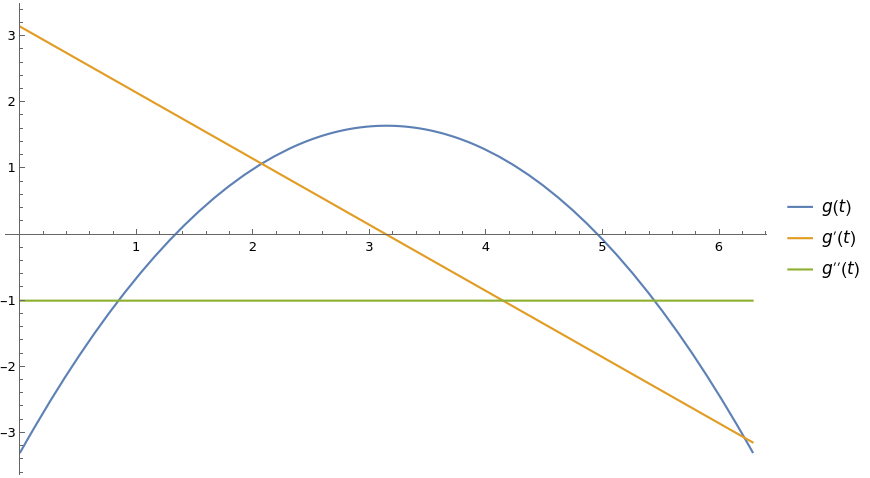
\includegraphics[width=10cm]{fourierplot.png}
  \caption{One Period of $g(t), g'(t)$, and $g''(t)$}
  \label{fig:1}
\end{figure}
\subsection*{Part 3}
First we need to see if this sum will converge in the distributional sense. The most important thing to notice is that $f(t)=g''(t)$. We know that the sum in $g(t)$ converges in the classical sense. This means it should converge in the distributional sense as well:
\begin{align*}
  -\sum_{n=-\infty,\neq0}^\infty\frac{e^{int}}{n^2}\quad\text{converges}
\end{align*}
We can also realize that if a distributional sum converges, so should its derivatives, not in the classical sense, but in the distributional sense, we can do this by realizing:
\begin{align*}
  \ip{g''(t)}{\phi(t)}=-\ip{g'(t)}{\phi'(t)}=\ip{g(t)}{\phi''(t)}
\end{align*}
And since $\phi\in C^\infty$, its second derivative is also a properly defined test function. Therefore this sum DOES converge. 
% We can identify $f(t)$ as the second derivative of $g(t)$, and $g(t)$ converges in the classical sense so it will converge in the distributional sense, hence $g''(t)$ converges in the distributional sense.

% As for what it will converge to we need to compute the following
% \begin{align*}
%   \ip{f(t)}{\phi(t)}&=\int_{-\infty}^\infty f(t)\phi(t)\dd{t}\\
%   &=\int_{-\infty}^\infty\sum_{-\infty}^{\infty} e^{int}\phi(t)\dd{t}\\
% \end{align*}
% We know the convergence of the sum as the second derivative of $g(x)$, and we would pick up 2 derivatives on $\phi$:
% \begin{align*}
%   \int_{-\infty}^\infty\sum_{-\infty}^{\infty} e^{int}\phi(t)\dd{t}&=
%   \int_{-\infty}^\infty\qty(-1-2\pi\sum_{k=-\infty}^\infty\delta(t-2k\pi))
%   \phi''(t)\dd{t}\\
%   &=-\int_{-\infty}^\infty\phi''(t)\dd{t}-2\pi\sum_{-\infty}^\infty\phi''(2k\pi)
% \end{align*}
% We found an identity for the sum in class:
% \begin{align*}
%   -\int_{-\infty}^\infty\phi''(t)\dd{t}-2\pi\sum_{-\infty}^\infty\phi''(2k\pi)&=
%   -\int_{-\infty}^\infty\phi''(t)\dd{t}-\int_{-\infty}^\infty\phi''(t)\dd{t}
%   -2\frac1\pi\sum_{k=1}^\infty\int_{-\infty}^\infty\cos(kt)\phi''(t)\dd{t}\\
%   &=-2\qty(\int_{-\infty}^\infty\phi''(t)\dd{t}
%   +\frac1\pi\sum_{k=1}^\infty\int_{-\infty}^\infty\cos(kt)\phi''(t)\dd{t})
% \end{align*}
% If we go back, the first term should be the zero distribution, so we only have the second term remaining
\section*{Problem 3}

\section*{Problem 4}
Using Gauss's Law, we have that the charge density and the electric field are related by:
\begin{align*}
  \div{\vb{E}}=\frac{\rho}{\varepsilon_0}
\end{align*}
The spherical coordinates divergence is given by:
\begin{align*}
  \div{\vb{A}}=\frac{1}{r^2}\pdv{(r^2\vb{A}\vdot\vu{r})}{r}
  +\frac1{r\sin\theta}\pdv{\theta}(\vb{A}\vdot\bm{\hat\theta}\sin\theta)
  +\frac1{r\sin\theta}\pdv{\vb{A}\vdot\bm{\hat\phi}}{\phi}
\end{align*}
The only non-zero dot product would be $\vb{E}\vdot\vu{r}$:
\begin{align*}
  \div{\vb{E}}&=\frac1{r^2}\pdv{r}\qty(r^2E_0H(a-r))\\
  &=\frac1{r^2}\qty(E_0r\qty(2H(a-r)-rH'(a-r)))\\
  &=\frac{E_0}{r}\qty(2H(a-r)-rH'(a-r))
\end{align*}
If we work in a distributional sense, we know the derivative of the Heaviside function $H$ is a $\delta$:
\begin{align*}
  \div{\vb{E}}&=\frac{E_0}{r}\qty(2H(a-r)-r\delta(a-r))
\end{align*}
Multiplying by $\varepsilon_0$ gives the charge density:
\begin{align}
  \boxed{
    \rho=\varepsilon_0\frac{E_0}{r}\qty(2H(a-r)-r\delta(a-r))
  }
\end{align}
The definition of total charge is the integral of the charge density over the volume:
\begin{align*}
  Q=\iiint\rho\dd{V}&=\int_0^{2\pi}\int_0^\pi\int_0^\infty
  \frac{E_0\varepsilon_0}{r}\qty(2H(a-r)-r\delta(a-r))r^2
  \sin\theta\dd{r}\dd{\theta}\dd{\phi}\\
  &=\varepsilon_0E_0\int_0^{2\pi}\int_0^\pi\int_0^\infty
  \qty(2rH(a-r)-r^2\delta(a-r))\sin\theta\dd{r}\dd{\theta}\dd{\phi}\\
  &=\varepsilon_0E_0\int\dd{\Omega}\int_0^\infty
  \qty(2rH(a-r)-r^2\delta(a-r))\dd{r}\\
  &=4\pi\varepsilon_0E_0
\end{align*}
T
\section*{Problem 5}
We can immediately move the laplacian over to the test function $\phi$:
\begin{align*}
  \ip{\laplacian{\ln(r)}}{\phi}=\ip{\ln(r)}{\laplacian{\phi}}
\end{align*}
There is a discontinuity at $r=0$ so we can write:
\begin{align*}
  \ip{\ln(r)}{\laplacian{\phi}}=\lim_{\epsilon\to0}
  \int_{\abs{r}>\epsilon}\ln(r)\laplacian{\phi}\dd{r}
\end{align*}
We want to make use of Green's Identity:
\begin{align*}
  \int\div{\vb{F}}\dd[2]{r}=\oint\vb{F}\vdot\vu{n}\dd{S}
\end{align*}
So that we end up with something of the form:
\begin{align*}
  \int\qty(\phi\laplacian{\psi}-\psi\laplacian\phi)\dd[2]{r}=
  \int\qty(\phi\grad{\psi}-\psi\grad{\phi})\vdot\dd{\vb{S}}
\end{align*}
We then take $\psi=\ln(r)$ and $\laplacian{\psi}=0$:
\begin{align*}
  \int\ln(r)\laplacian{\phi}\dd[2]{r}=\int(\ln(r)\grad\phi-\phi\grad{\ln(r)})
  \vdot\vu{n}\dd{S}
\end{align*}
We realize that $\vu{n}\vdot\gradient=\pdv{r}$ since we are using polar coordinates.
\begin{align*}
  \int(\ln(r)\grad\phi-\phi\grad{\ln(r)})\vdot\vu{n}\dd{S}=
  \int\qty(\ln(\epsilon)\pdv{\phi}{r}-\phi\frac{1}{r})
  r\dd{\varphi}
\end{align*}
The $\phi$ integration is what gives us the factor of $2\pi$, and in the same way as before we get a $\phi(0)$ by integrating by parts again:
\begin{align*}
  \ip{\laplacian{\ln(r)}}{\phi}=\ip{2\pi\delta}{\phi}
\end{align*}
Hence:
\begin{align}
  \boxed{
    \laplacian{\ln(r)}=2\pi\delta(r)
  }
\end{align}
\end{document}